\documentclass[twocolumn,superscriptaddress,aps]{revtex4-1}


%%%%%%%%%%%%
% Packages %
%%%%%%%%%%%%

\usepackage[utf8]{inputenc}

\usepackage{amsfonts}
\usepackage{amssymb}
\usepackage{amsmath}
\usepackage{amsthm}

\usepackage{bbold}
\usepackage{bm}
\usepackage{graphicx}
\usepackage{color}
\usepackage{hyperref}


%%%%%%%%%
% Setup %
%%%%%%%%%

\setlength{\parindent}{0pt}


%%%%%%%%%%%%
% Document %
%%%%%%%%%%%%

\begin{document}
    % ----- Information ----- %
    \title{\Large{INFO8010 : Project proposal}}
    \vspace{1cm}
    
    \author{\small{\bf Maxime Meurisse}}
    \affiliation{\texttt{m.meurisse@student.uliege.be} (\texttt{s161278})}
    
    \author{\small{\bf Adrien Schoffeniels}}
    \affiliation{\texttt{adrien.schoffeniels@student.uliege.be} (\texttt{s162843})}
    
    \author{\small{\bf Valentin Vermeylen}}
    \affiliation{\texttt{valentin.vermeylen@student.uliege.be} (\texttt{s162864})}

    % ----- Title ----- %
    \maketitle
    
    % ----- Description and motivation ----- %
    \section{Description and motivation}
    
    For this deep learning project, we have decided to try to tackle the task of \textbf{neural style transfer}. The goal of such a task is to combine the content and style of two different images.\\
    
    An example of such a feat is provided at figure \ref{fig:example}.
    
    \begin{figure}[h]
        \centering
        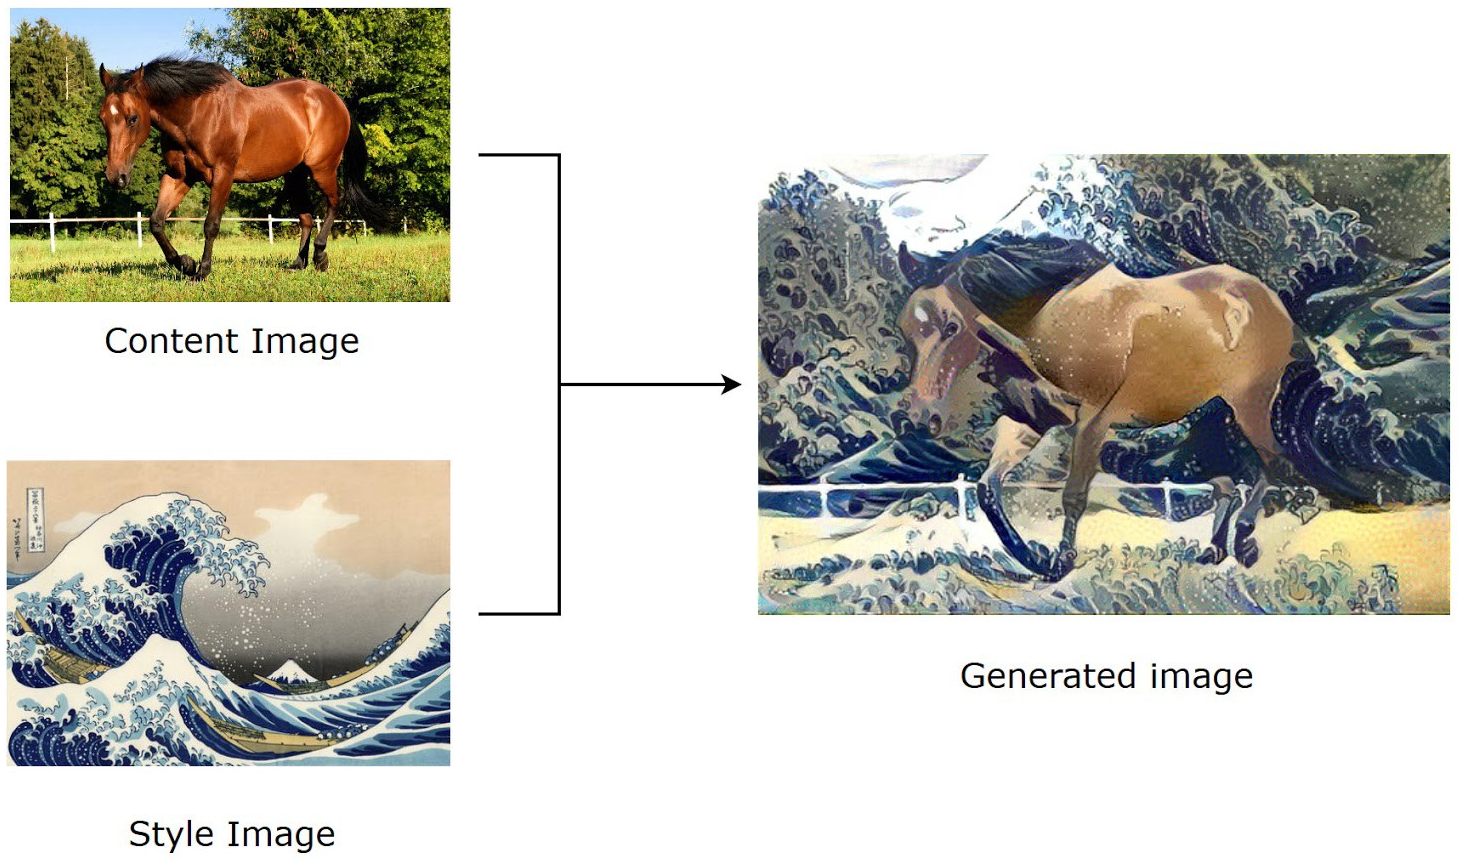
\includegraphics[width=0.45\textwidth]{resources/png/example.png}
        \caption{An example of neural style transfer product \cite{towards-data-science-img}.}
        \label{fig:example}
    \end{figure}
    
    There are several reasons why we chose this task.\\
    
    Firstly, we think that a visual output (or at least an output that can be made visual) was more appealing than a more abstract one. Also, with this kind of task, we will not have to wait hours or close to the end of the project to see if the results are satisfactory or not (unlike with some recurrent neural networks).\\
    
    Secondly, there exists some papers tackling this task on which we can base our work and, among some other project propositions, this was the one Mr Sabatelli advised us to take and was the most enthusiastic about. So we have a lot of resources at our disposal.\\
    
    Finally, we believe satisfactory results can be obtained with the limited time we will have to dedicate to this project. Indeed, in view of our still weak knowledge in the field and the other projects we must work on in parallel, we preferred to choose a project where we will be able to achieve results and present a complete and accomplished work within the allotted time.
    
    % ----- Data acquisition ----- %
    \section{Data acquisition}
    
    For one style, we only need one style image but a lot of content images. Those content images do not need to have any specific characteristics, they will only be used to train our neural network and can thus be random copyright-free images found on the internet.\\
    
    Style images will be photographs of famous artworks or images with an interesting style.\\
    
    There are a large number of free image databases from which we can draw our resources. For example, just to name a few, \textcolor{blue}{\href{http://www.image-net.org}{ImageNet}}, \textcolor{blue}{\href{https://github.com/openimages/dataset}{Open Images Dataset}}, \textcolor{blue}{\href{http://www.cs.toronto.edu/~kriz/cifar.html}{CIFAR-10}} or simply \textcolor{blue}{\href{https://www.google.com/imghp}{Google Images}} (with an appropriate API to automatically download images).
    
    % ----- Computing resources ----- %
    \section{Computing resources}
    
    Our research did not lead us to precise figures regarding the resources and time we will need to train our models.\\
    
    This will depend on the number of images in our dataset and the training time we will use. Several sources indicate that it is possible to get results quickly, but these are based on a very small dataset (or already use a pre-trained model).\\
    
    We think it would be technically possible to train our models in a reasonable way on our machines, but if the Montefiore Institute has a GPU cluster that we could take advantage of, it would be an opportunity for us to take the project further and certainly get much better results.
    
    % ----- Nice-to-have ----- %
    \section{Nice-to-have}
    
    Our primary goal is to obtain a neural network capable of applying the style of one image to the content of another image. Unlike some other projects, we do not think this task has several incremental goals that are reachable. Either we are able to design and train a neural network to perform neural style transfer or not.\\
    
    If we have time, we would like to try to apply this model to video processing. We could also try to handle real-time processing.\\
    
    As a bonus, we would like to compare the technique called "optimization" and the "feedforward" one presented in the article \cite{medium-neural-artistic-style-transfer}, and/or the difference between the results obtained from a neural network and those not obtained from neural networks, as described in the paper \cite{1705-04058}.
    
     % ----- Related works ----- %
    \section{Related works}
    
    Once we had decided to tackle this task, we looked in the literature for papers or links concerning this problem and found some from which we will take inspiration and/or will try to recreate and retrain the models. These sources, as of today, are the following : \\
    
    \cite{1508-06576} : a paper written by Leon A. Gatys, Alexander S. Ecker and Matthias Bethge which seems to be the original paper for the task of neural style transfer. Its sets the base for the task.\\
    
    \cite{github-neural-style-transfer} : a Github repository implementing the paper cited just above.\\
    
    \cite{tensorflow-style-transfer} : a Tensorflow tutorial about neural style transfer.\\
    
    \cite{1705-04058} : this paper provides an overview of the current progress towards NST and a comparison between the approaches. This paper can serve as a starting point to choose the algorithm we will implement and to provide ideas for improvements.
    
    % ----- Bibliography ----- %
    \bibliographystyle{unsrt}
    \bibliography{sources.bib}
\end{document}
